\documentclass{beamer}
\usepackage[utf8]{inputenc}

\usetheme{Antibes}

\title
  [Sistema de Recomendação Baseado em Confiança para Promover a Colaboração em Redes de Pesquisa Científica]
  {TFG I - Proposta}
\subtitle{Sistema de Recomendação Baseado em Confiança para Promover a Colaboração em Redes de Pesquisa Científica}
\author[João Pedro Raskopf, Fernando Prass]{J.P.~Saldanha\inst{1} \and F.~Prass\inst{1}}
\institute[Some University]
{
  \inst{1}%
  Ciência da Computação\\
  Universidade Fransicana
} 
\date[Proposta TFG]{Jul. 2019 / TFG I}

\begin{document}

\begin{frame}
  \titlepage
\end{frame}

\section{Introdução}

\begin{frame}{Resumo}{}
  
  \begin{itemize}
    \item Sistema de Recomendação
    \begin{itemize}
      \item Promover Colaborações
    \end{itemize}
  \end{itemize}

  \begin{itemize}
    \item Usuários
    \begin{itemize}
      \item Pesquisadores
    \end{itemize}
  \end{itemize}
  
  \begin{itemize}
    \item Metodologia
    \begin{itemize}
      \item Método Baseado em Conteúdo
      \item Método Baseado em Confiança
    \end{itemize}
  \end{itemize}

  \begin{itemize}
    \item Dados
    \begin{itemize}
      \item Plataforma Lattes
      \item Plataforma Kennis
    \end{itemize}
  \end{itemize}

\end{frame} 

\begin{frame}{Pesquisa Ciêntifica}{}
  
  \begin{itemize}
    \item Incrementar o Conhecimento
    
    \begin{itemize}
      \item Referências
      \item Colaborações
    \end{itemize}
    
    \item Não reinventar a roda
    \item "Stand on the Shoulders of Giants" - Google Acadêmico
  \end{itemize}

\end{frame}

\begin{frame}{Plataforma Lattes}{}
  
  \begin{itemize}
    \item Base de dados de Curriculos
  \end{itemize}

  \begin{block}{CNPq}
    "Padrão nacional  no  registro  da  vida pregressa e atual dos estudantes e pesquisadores do país"
  \end{block}

\end{frame}

\begin{frame}{Sobrecarga de Informações}{}

  \begin{itemize}
    \item Em um ano... 
    \begin{itemize}
      \item 2.5 milhões de artigos por ano
      \item Aumento de 5\% no número de autores 
    \end{itemize}

    \item Impossível considerar
    \begin{itemize}
      \item Relacionados
      \item Linhas de pesquisa
      \item Pesquisadores 
    \end{itemize}

    \item Trabalho repetido
    \item Perda da oportunidade de colaborações 

  \end{itemize}

\end{frame}

\begin{frame}{Sistemas de Recomendação}{}

  \begin{itemize}
    \item Pessoas tendem a considerar recomendações de amigos/especialistas
    \item Analisar têndencias dentro de comunidades
    \item Filtragem das informações/itens em websites
  \end{itemize}

\end{frame}

\subsection[Objetivos]{}

\begin{frame}{Objetivos}{}

  \begin{block}{Geral}
    Promover a colaboração de pesquisadores em trabalhos ciêntificos
  \end{block}

  \begin{itemize}
    \item Estudar funções e aplicações de sistemas de recomendação
    \item Modelar a rede de confiança da comunidade científica
    \item Estabelecer métricas de confiança para os dados disponíveis
    \item Estimar a confiança entre os pesquisadores 
    \item Pré-selecionar recomendações
    \item Filtrar a pré-seleção com a confiança computada
    \item Avaliar o modelo
  \end{itemize}

\end{frame}

\begin{frame}{Proposta}{}

  \begin{itemize}
    \item Descrever uma rede de colaborações
    \item Computar a propagação de confiança na rede 
    \item Pré-seleção dos itens com o método baseado em conteúdo
    \item Arquitetura para o sistema de recomendações
  \end{itemize}

\end{frame}

\subsection[Revisão Bibliográfica]{}

\begin{frame}{Sistemas de recomendação (SR)}{}

  \begin{itemize}
    \item Filtrar a grande quantidade de itens das plataformas
    \item Predizer a relevância do Item
    
    \item Usuários
      \begin{itemize}
        \item $ u_1, ... u_n \in U $
      \end{itemize}

    \item Itens
      \begin{itemize}
        \item $ i_1, ... i_n \in I$
      \end{itemize}
    
    \item Relações
      \begin{itemize}
        \item Onotlogia
        \item Matriz $ |U| \times |I| $
      \end{itemize}
    
    \item Função de predição
      \begin{itemize}
        \item Real: $ f (u, i) $
        \item Computada: $\hat{f}(u, I)$
      \end{itemize}
  \end{itemize}
\end{frame}

\begin{frame}{Tipos de SR}{}
  \begin{block}{Filtragem Colaborativa}
    Itens bem avaliados pelos vizinhos serão também avaliados positivamente pelo usuário alvo, já que os perfis são semelhantes
  \end{block}
  %Problema da primeira avaliação
  \begin{block}{Baseado em Conteúdo}
    Usuários têm interesse em itens semelhantes àqueles que lhe foram uteis no passado
  \end{block}
  %Mais pesado, Não se recomenda coisas novas
  \begin{block}{Baseado em Confiança}
    O usuário recebe recomendações de itens avaliados positivamente por usuários em sua rede de confiança
  \end{block}
  %Metodos Híbridos
\end{frame}

\subsection[Trabalhos Relacionados]{}

\begin{frame}{Desenvolvimento de um Sistema de Recomendação para Bibliotecas Digitais}
  {Furlan et al. 2018}
  
  \begin{itemize}
    \item Aborda o problema da sobrecarga de informações 
    \begin{itemize}
      \item Baseando-se no perfil do currículo Lattes
    \end{itemize}

    \item Aborda o problema da sobrecarga de informações 
    \begin{itemize}
      \item Filtragem colaborativa \& Baseado em conhecimento
      \item Problema da primeira avaliação
    \end{itemize}
  \end{itemize}
\end{frame}

\begin{frame}{Técnicas de Recomendação para usuários de Bibliotecas Digitais}
  {Primo \& Loh 2006}
  
  \begin{itemize}
    \item Apresentam técnicas populares de recomendação 
    \item Abordagens para a elaboração de um SR de obras literárias
    \item SR Híbrido
    \item Comparativo das metodologias usadas
  \end{itemize}
\end{frame}

\begin{frame}{Trust-aware Collaborative Filtering for Recommender Systems}
  {Massa \& Avesani 2004}
  
  \begin{itemize}
    \item Melhorar sugestões em SRs usando métricas de confiança 
    \item Distância mínima entre nós
    \item PageRank como métrica global
    \item Arquitetura com módulos substituíveis
  \end{itemize}
\end{frame}

\section{Materiais \& Métodos}

\subsection{Introdução}

\begin{frame}{Materiais \& Métodos}{}

  \begin{itemize}
    \item Estimar a confiança entre pesquisadores
    \begin{itemize}
      \item Modelar uma rede de confiança
      \item Local ou global
    \end{itemize}
    \item Selecionar potenciais colaboradores baseando-se no perfil
    \item Ordenada de acordo com a confiança estimada
  \end{itemize}
\end{frame}

\subsection{Dados}

\begin{frame}{Os Dados da Plataforma Lattes}{}

  \begin{itemize}
    \item Plataforma Kennis
    \begin{itemize}
      \item Parser do currículo Lattes
      \item Limpeza e pré-processamento
    \end{itemize}
    \item Banco de dados relacional
  \end{itemize}

\end{frame}

\begin{frame}{Diagrama ER}{}
  \begin{figure}[ht]
    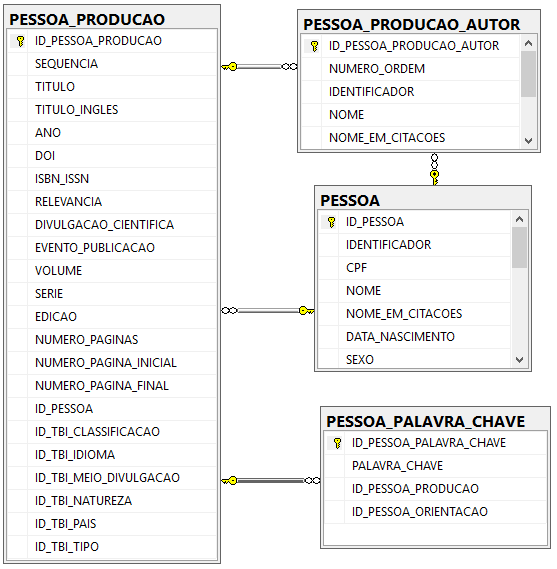
\includegraphics[width=.65\textwidth]{database.png}
  \end{figure}
\end{frame}

\subsection{Computando Confiança}

\begin{frame}{Rede de Publicações}{}

  \begin{itemize}
    \item Rede de confiança
    \begin{itemize}
      \item Nodos: Pesquisadores
      \item Arestas: publicações em conjunto
    \end{itemize}
    \item Propagação \& Agregação de confiança
  \end{itemize}
  
\end{frame}

\begin{frame}{Rede de Confiança}{}
  \begin{figure}[ht]
    \includegraphics[width=1.05\textwidth]{trust-network.png}
  \end{figure}
\end{frame}

\begin{frame}{PageRank}
  {Page et al. 1999}

  \begin{itemize}
    \item Ranking global de citações
    \item Dissipação de ranking 
    \begin{itemize}
      \item Seja $R$ o ranking de uma página qualquer, $u$
      \item $R$ é a soma dos rankings dissipados pelas paginas que referenciam $u$($B_u$)
      \item $R$ é distribuído igualmente entre as páginas as quais $u$ faz referência ($F_u$)
    \end{itemize}
  \end{itemize}
\end{frame}

\begin{frame}{PageRank}{}

  \begin{itemize}
    \item Matriz de adjacência
    \begin{equation} \label{eqn:adjacency-matrix}
      \hat{A}_{u,v} =
       \begin{cases}
         1       & \quad \text{se } \text{ há links de u para v}\\
         0       & \quad \text{se } \text{ não há links de u para v}
       \end{cases}
   \end{equation}
   \item $A = \frac {\hat{A}} {|F|}$
   \item $R = c(AR + E)$
  \end{itemize}
\end{frame}

\begin{frame}{PageRank}{}

  \begin{itemize}
    \item \textit{"A aplicação de PageRank à um grafo não-direcionado gera um vetor $R$ estatisticamente similar à distribuição de grau dos nodos da rede"}
    \item No final das contas a confiança seria proporcional ao número de publicações do autor
    \item Não é considerada a confiança dos colaboradores, somente o valor total de colaborações
  \end{itemize}
\end{frame}

\begin{frame}{Relevância}{}
  \begin{table}[ht]
    \label{tab:relavancy}
    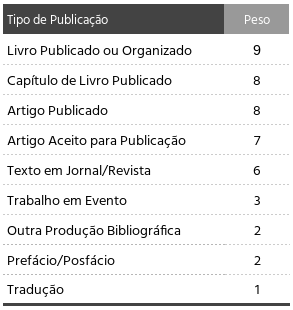
\includegraphics[width=.5\textwidth]{heuristics.png}
  \end{table}
\end{frame}

\begin{frame}{Centralidade}{Opsahl et al. 2010}
  \begin{itemize}
    \item Seguir a ideia de \textit{PageRank} 
    \item Cálculo da centralidade dos nodos. 
    \item  Relevância \& quantidade de colaborações devem ser levadas em consideração na distribuição de confiança.     
  \end{itemize}
\end{frame}

\begin{frame}{Centralidade}{Opsahl et al. 2010}
  \begin{equation} \label{eqn:centrality} 
    C_D ^{w \alpha} (i) = k_i ^{1 - \alpha} \times s _i ^{\alpha}
  \end{equation}
  \begin{table}[ht]
    \label{tab:centrality}
    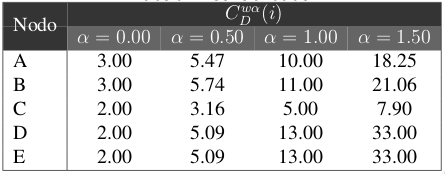
\includegraphics[width=.8\textwidth]{centrality.png}
  \end{table}
\end{frame}

\begin{frame}{Distância}{Opsahl et al. 2010}
  \begin{itemize}
    \item Confiança local 
    \item Distância entre os Pesquisadores
    \item Amigos de Amigos
    \item Mais facilidade para realizar colaborações
    \item Cálculo da Distância dos nodos
    \item Algoritmo de Dijikstra
    \item os pesos representam força dos laços
  \end{itemize}
\end{frame}

\begin{frame}{Distância}{Opsahl et al. 2010}
  \begin{equation} \label{eqn:distance}
    d^{w\alpha}(i, j) = min \left( \frac{1}{ \left( w_{ih}^{\alpha} \right) } + \dots + \frac{1}{ \left( w_{hj}^{\alpha} \right) }  \right) 
  \end{equation}
  \begin{table}[ht]
    \label{tab:distances}
    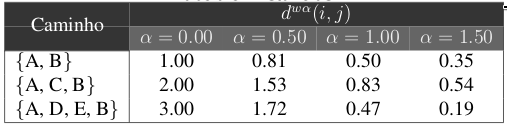
\includegraphics[width=.85\textwidth]{distances.png}
  \end{table}
\end{frame}

\begin{frame}{Pré-seleção de Recomendações}{}
  \begin{itemize}
    \item Apenas confiança pode não ser suficiente para recomendações de qualidade
    \item Considerar também a linha de pesquisa do pesquisador
    \item Pré-seleção dos itens utilizando um método baseado em conteúdo
    \item Técnica de vetorização \textit{TF-IDF}
    \begin{itemize}
      \item Semelhança entre termos
    \end{itemize}
    \item Sklearn
  \end{itemize}
\end{frame}

\subsection{Arquitetura}

\begin{frame}{Arquitetura do SR}{Massa \& Avessani}
  \begin{figure}[ht]
    \includegraphics[width=1\textwidth]{SR-arch.png}
    \label{fig:sr-arch}
  \end{figure}
\end{frame}

\subsection{Validação}

\begin{frame}{Validação}{Feedback dos usuários}
  \begin{itemize}
    \item Estaria ele interessado em colaborar com o pesquisador recomendado ?
    \item Qual a facilidade de iniciar a colaboração ?
    \item Qual a confiança do usuário no pesquisador responsável ?  
  \end{itemize}
\end{frame}

\section{Conclusão}

\begin{frame}{Conclusão}{}
  \begin{itemize}
    \item É possível estender o trabalho com melhores heurísticas
    \begin{itemize}
      \item Data de publicação
      \item Eventos
    \end{itemize}
    \item Incorporar mais métricas  
    \begin{itemize}
      \item Global
      \item Local
    \end{itemize}
  \end{itemize}
\end{frame}

\section{}

\begin{frame}
  \titlepage
\end{frame}

\end{document}
